\appendix


\chapter{An efficient method to update the COHSEX self--energy during the time evolution}
%%%%%%%%%%%%%%%%%%%%%%%%%%%%%%%%%%%%%%%%%%%%%%%%%%%%%%%%%%%%%%%%%%%%%%%%%%%%%%%%%%%%%%%%%%
\label{fastcohsex}
In this appendix we show how we store and update the $\Sigma^{\text{cohsex}}$ self-energy in a efficient manner. First of all we neglect the variation of the
screened interaction $W(\mathbf r,\mathbf {r'}; G^<(t))$ with respect to the $G^<(\mathbf r,\mathbf{r'},t)$ by setting to zero the functional
derivative $\partial W/\partial G$ (see Sec.~\ref{linear_response}). Within this approximation the $\Sigma^{\text{coh}}$ does not contribute to the
time evolution, therefore only $\Sigma^{\text{sex}}$ needs to be updated:
\begin{align}
\Sigma^{\text{sex}}(\mathbf r,\mathbf{r'},t) = i W(\mathbf r,\mathbf {r'})\sum_{\substack{n,n'}{\kk}} \varphi^{}_{n, \kk}(\mathbf r) 
\varphi^*_{n', \kk}(\mathbf {r'}) G^<_{n,n',\kk}(t).
\label{sex}
\end{align} 
The KBE
%%Baym--Kadanoff equation ??? Which convention do we choose?
involves the  matrix elements $ \langle m, \kk |\Sigma^{sex} | m', \kk \rangle$:
\begin{align}
\Sigma^{\text{sex}}_{m,m',\kk}(t) = \sum_{\substack{\mathbf G,\mathbf{G'},\mathbf q \\ n,n'}} \rho^{}_{\substack{m,n \\ \mathbf{k,q}}} (\mathbf{G'})
\rho^*_{\substack{m',n' \\ \mathbf{k,q}}}(\mathbf{G}) W_{\mathbf G,\mathbf G'}(\mathbf q) G^<_{\substack{n,n' \\ \mathbf{k-q}}}(t),
\end{align}
where 
\be
\rho^{}_{\substack{m,n \\ \mathbf{k,q}}} (\mathbf{G}) = \int  \varphi^*_{m, \kk}( \mathbf r) \varphi_{n,\mathbf{k-q}}( \mathbf r)  e^{i(\mathbf G+\mathbf q) \mathbf r}.
\ee
In order to rapidly update  $\Sigma^{\text{sex}}$ after a variation of  $G^<(\mathbf r,\mathbf{r'},t)$, we store the matrix elements:
\be
M_{ \substack{m,m',n,n' \\ \mathbf q, \kk}} =  \sum_{\mathbf G,\mathbf {G'}} \rho^{}_{m,n} (\kk,\mathbf q,\mathbf{G'}) \rho^*_{m',n'}( \kk, \mathbf q,
\mathbf G) W_{\mathbf G,\mathbf G'}( \mathbf q ) ,
\ee
in such a way that $\Sigma^{\text{sex}}_{m,m'}$ can be rewritten as
\be
\Sigma^{\text{sex}}_{m,m',\kk}(t) = \sum_{\substack{n,n' \\ \mathbf{q}}} M_{\substack{m,m',n,n' \\ \mathbf q, \kk}} \cdot G^<_{\substack{n,n' \\
\mathbf{k-q}}}(t).
\ee
The $M$ matrix can be very large, but its size can be reduced by noticing that: 
(i) the matrix $M$ is Hermitian respect to the $(m,m')$ indexes; 
(ii) the number of {\bf k} and {\bf q} points is reduced by applying the operation symmetries that are left unaltered by the applied external
field; (iii) for converging optical properties only the bands close to the gap are needed.
As an additional numerical simplification we neglected all terms such that $M_{ \substack{m,m',n,n' \\ \mathbf q,\kk}} /\max\{ M_{ \substack{ m,m',n,n'
\\ \mathbf q , \kk}}\}<M_c$, where $M_c$ is a cutoff that, if chosen to be $M_c \simeq 5\cdot 10^{-3}$  does not appreciably affect the final results. In principle by using an auxiliary localised basis set\cite{schwegler:9708,faber2014excited} one can obtain a further reduction of the matrix dimensions, but in the present work we did not explore this strategy.



\chapter{Induced field and response functions} \label{appA}
%********************************************************

One of the objectives of atomistic simulations is the calculation of
the macroscopic dielectric function or of related response functions of dielectrics.
Within TD-DFT such goal is achieved via the calculations of the
microscopic density--density response function $\tchirr$, defined via the equation
\be
\delta n_{\sss \GG}(\qq,\w)=\tchirr_{\sss \GG\GG'} (\qq,\w)\ \delta v^{\text{ext}}_{\sss \GG'} (\qq,\w).
\label{eq:chi_red} 
\ee
Here $\GG$ are the reciprocal lattice vectors and $\w$
the frequency obtained from the Fourier transforms $\rr\ra\GG$ and $t\ra\w$.
In addition to  $\tchirr$, 
 the irreducible response function $\chirr$ and
 the auxiliary response function $\bchirr$ can be defined via
 \bea
 \delta n_{\sss \GG}(\qq,\w)&=&\chirr_{\sss \GG\GG'}(\qq,\w)\
  \delta v^{\text{tot}}_{\sss \GG'}(\qq,\w) \label{eq:chi_irr} \\
  \delta n_{\sss \GG}(\qq,\w)&=&\bchirr_{\sss \GG\GG'} (\qq,\w)
   [\delta v^{\text{ext}}_{\sss \GG'}(\qq,\w)+\delta \bar v^\text{H}_{\sss \GG'}(\qq,\w)]. \label{eq:chi_bar}
   \eea

   To linear order and at finite momentum (i.e. $\qq\neq\zero$),
   the longitudinal microscopic dielectric function can be derived from the response functions,
   \bea
   \epsilon^{-1}_{\sss \GG\GG'}(\qq,\w)=\delta_{\sss \GG,\GG'}
     + 4\pi \frac{\tchirr_{\sss \GG\GG'}(\qq,\w)}{|\qq+\GG||\qq+\GG'|}
     \label{eq:eps_M1_micro} , \\
     \epsilon_{\sss \GG\GG'}(\qq,\w)=\delta_{\sss \GG,\GG'}
       - 4\pi \frac{\chirr_{\sss \GG\GG'}(\qq,\w)}{|\qq+\GG||\qq+\GG'|}
       \label{eq:eps_micro}
       \text{.}
       \eea
       The longitudinal macroscopic dielectric function can then be obtained as
       $\epsilon_M(\qq,\w)=1/\epsilon^{-1}_{\sss \zero\zero}(\qq,\w)$.
       Absorption experiment however are described at $\qq=\zero$
       where the dielectric function 
       $\epsilon_M(\w)\equiv \epsilon_M(\zero,\w)$
       can be obtained only via a limiting process.
       They are defined as
       \bea
       \epsilon_M(\w)&=&\left[ 1 + 4\pi\lim_{\qq\ra 0} \frac{\tchirr_{\sss \zero\zero}(\qq,\w)}{|\qq|^2}\right]^{-1} \\
       \epsilon_M(\w)&=&\      1 - 4\pi\lim_{\qq\ra 0} \frac{\bchirr_{\sss \zero\zero}(\qq,\w)}{|\qq|^2}
       \text{.}
       \eea
       As we observed in the introduction this approach is at least problematic in real time simulation,
       where it is numerically more convenient to directly work at $\qq=0$ and thus the density--density
       response function cannot be used.

       Within DPFT the key quantity is the one which relates the macroscopic electric
       field $\Efield^{tot}$ or $\Efield^{ext}$ to the first order polarisation $\PPo 1$.
       \bea
       \PPo 1(\w)=\newtensor{\tilde{\chi}}(\w) \Efield^{ext}(\w) \label{eq:tsusc1} \\
       \PPo 1(\w)=\newtensor{       \chi }(\w) \Efield^{tot}(\w)  \label{eq:susc1}     
       \text{.}
       \eea
       $\newtensor{\chi}(\w)=\newtensor{\chi}^{(1)}(\w)$ is the (first--order) polarizabilty;
       $\newtensor{\tilde{\chi}}(\w)=\newtensor{\tilde{\chi}}^{(1)}(\w)$ is the quasi--polarizability.
       Since we obtain the polarizability dividing the Fourier transform of the time--dependent
       polarisation with the input electric field, we obtain either
       $\newtensor{\tilde{\chi}}(\w)$ or $\newtensor{\chi}(\w)$
       depending on whether we divide by $\Efield^{\text{ext}}$ or $\Efield^{\text{tot}}$.
       Notice that in this framework we have already made the distinction between macroscopic fields,
       described in terms of $\Efield^{\text{ext}}/\Efield^{\text{tot}}$, and microscopic ones,
       described in terms of $\bar v^{\text{tot}}/\bar v^{\text{tot}}$.
       $\newtensor{\tilde{\chi}}(\w)$ and $\newtensor{\chi}(\w)$
       are thus macroscopic functions.
       %\\
       %{\color{red} Davide: Here there is still something to be fixed because in the literature
       %$\susc 1$ and $\tsusc 1$ are defined in terms of the external and the perturbing field
       %[See PRB Fiorino and Del Sole]. Instead here we are using the total field. The 
       %perturbing field contains only the induced longitudinal term, in $\chirr$ everything is
       %longitudinal and there is no need of such distinction ... maybe also in the $\qq\ra 0$ limit.} \\
       The longitudinal dielectric function can be obtained, to first order in the field, as
       \bea
       \epsilon_M(\w) &=& \left[ 1 + \tilde{\chi}_{ii}(\w)\right]^{-1}, \\
       \epsilon_M(\w) &=&\       1 -        \chi_{ii}(\w),
       \eea
       where $\tilde{\chi}_{ii}$ is any of the diagonal components of $\newtensor{\chi}$.

       More in general the $n$-order polarisation can be expressed as
       %\bea\label{eq:PpwrfE}
       %\PP(t) =& \int dt_1 \susc 1(t;t_1)\Efield(t_1) \\ 
       %+& \iint dt_1 dt_2 \susc 2(t;t_1,t_2)\Efield(t_1)\Efield(t_2) + \dots \nonumber \\
       %+& \iiint dt_1 dt_2 dt_3 \susc 3(t;t_1,t_2,t_3)\Efield(t_1)\Efield(t_2)\Efield(t_3) + \dots\\
       %\PPo 1(t)&=& \int dt_1 \susc 1(t-t_1)\Efield^{\text{tot}}(t_1) \\ 
       %\PPo 2(t)&=& \iint dt_1 dt_2 \susc 2(t-t_1,t-t_2)\times \nonumber \\ 
       %         &&\phantom{dt_1 dt_2} \Efield^{\text{tot}}(t_1)\Efield^{\text{tot}}(t_2) ,  \\
       %.. \nonumber \\
       %\eea
       \begin{multline}\label{eq:PpwrfE}
               \PPo n(t)= \int dt_1\ ...\ dt_n\times \\ \susc n(t-t_1,\ ...\ ,t-t_n)\times  \\ 
                        \Efield^{\text{tot}}(t_1)\ ...\ \Efield^{\text{tot}}(t_n) ,
                \end{multline}
                where $\susc n$ is the $n$-order polarizability related to $n$-order nonlinear
                optical properties.
                Also here we could define the $\tsusc n$ as the response to the external field.
                The two can be related from the equation
                \be
                \tsusc n(\w)=\susc n(\w)(1-\susc 1)^n
                \ee
                As for the linear case we obtain either $\tsusc n(\w)$ ot $\susc n(\w)$
                depending for whether field we divide the polarisation $\Efield^{ext}$ or $\Efield^{tot}$.
                However, since usually $\susc n(\w)$ is the quantity considered in the literature the
                last choice is more convenient in nonlinear optics.

In practice, in real-time simulations we can choose to provide as input field  the total $\Efield^{tot}$ or the external one $\Efield^{ext}$.
In the first case we propagate the equation:
\be
i\hbar  \frac{d}{dt}| v_{m\kk} \rangle = \left( H^{\text{mb}}_{\kk} +i \Efield^{tot} \cdot \tilde \partial_\kk\right) |v_{m\kk} \rangle,
\ee
while in the second case we propagate the coupled Sch\"odinger plus Maxwell equations:
\bea
\left\{
\begin{array}{cc}
    i\hbar  \frac{d}{dt}| v_{m\kk} \rangle = \left( H^{\text{mb}}_{\kk} +i \Efield^{tot} \cdot \tilde \partial_\kk\right) |v_{m\kk} \rangle   \\
    \Efield^{tot} =  \Efield^{ext} + 4 \pi \PP.  
\end{array}
\right.
\eea
In this last case the total field is generated directly by the Maxwell equation. Since response functions are independent from the field, the two formulations provide the same response functions. However in numerical simulations, the first approach is preferable because we know analytically the total field. This allow us to have less numerical noise while extracting the $\susc n(\w)$ coefficients and we can probe precisely the frequencies we are interested in. 

\begin{figure}[h]
\centering
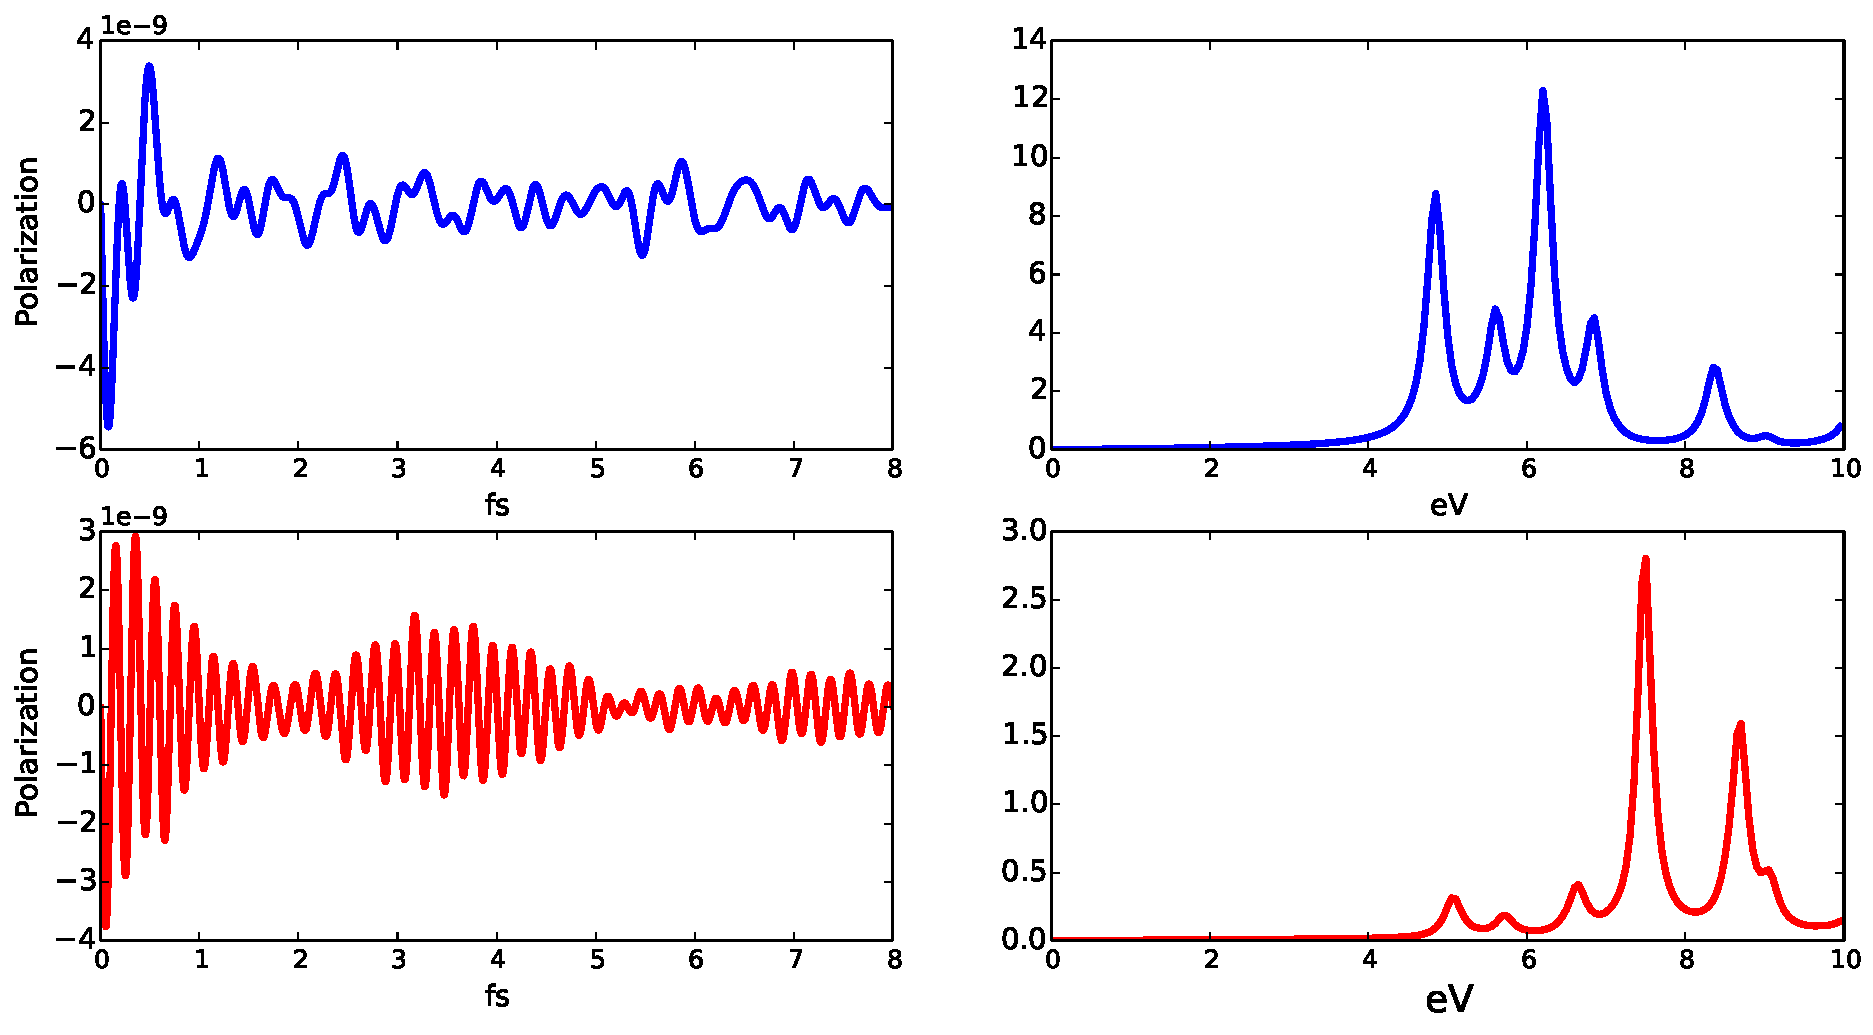
\includegraphics[width=0.7\textwidth]{Figures/pol_eps_and_eels.pdf}
\caption{\footnotesize{Polarisation, dielectric constant and EELs in hexagonal-BN at IPA. We excite the system with a delta function electric field at $\Efield^{inp} = \mathcal{E}_0 \delta(t)$. (top left) The real-time polarisation obtained using $\Efield^{tot} = \Efield^{inp}$, (bottom left) the polarisation obtained using $\Efield^{ext} = \Efield^{inp}$. (top right) The dielectric constant, (bottom right) the EELS.}\label{induced}}
\end{figure}  

Nevertheless if one is interested in quantities that depend from the field intensity, as for instance electro-absorption, saturation etc.. the correct formulation is the second one. In fact in a real material electrons cannot couple directly to the external field but they couple to the sum the external plus the field generated by the electron them-self. For a discussion on this point and a more rigorous treatment see Ref.~\cite{PhysRevB.85.045134}.\\
As example of these two formalisms let's consider the case of an insulator  subject to a delta function field,   $\Efield^{inp} = E_0 \delta(t)$, in independent particle approximation. If you use $\Efield^{inp}$ as the total one, the polarisation will oscillate according to the electron-hole frequencies, while if we couple the Sch\"odinger equation to the Maxwell one the polarisation will oscillate according to the plasmon frequencies, as depicted in Fig.~\ref{induced}. This can be easily understood from Eq.~\ref{eq:tsusc1} and \ref{eq:susc1}. In the first case the polarisation divided by the total field (that is a constant) is proportional to the EELs, while in the second case dividing the polarisation for the external one gives directly the dielectric constant. This explain the different behaviour of the polarisation in the two cases.  
\chapter{List of publications}
\begin{itemize}
    \item \emph{Optical properties of periodic systems within the current-current response framework: numerical pitfalls and solutions}\\
        D. Sangalli, J. A. Berger, C. Attaccalite, M. Gr\"uning and P. Romaniello, in preparation (2016) 
    \item \emph{Excitonic effects in third harmonic generation: the case of carbon nanotubes and nanoribbons}\\
        C. Attaccalite, E. Cannuccia and M. Gr\"uning, in preparation (2016) 
    \item \emph{Dielectrics in a time-dependent electric field: A real-time approach based on density-polarization functional theory}\\ M. Gr\"uning, D. Sangalli, and C. Attaccalite, Phys. Rev. B \textbf{94}, 035149 (2016)
    \item \emph{Performance of polarisation functionals for linear and nonlinear optical properties of bulk zinc chalcogenides ZnX (X = S, Se, and Te)}\\
        M. Gr\"uning and   C. Attaccalite, Phys. Chem. Chem. Phys., \textbf{18}, 21179 (2016) 
    \item \emph{Optical properties of Cu-chalcogenide photovoltaic absorbers from self-consistent GW and the Bethe-Salpeter equation} \\
        Sabine K\"orbel, David Kammerlander, Rafael Sarmiento-P\`erez, Claudio Attaccalite, Miguel A. L. Marques, and Silvana Botti, Phys. Rev. B \textbf{91}, 075134 (2015)
    \item \emph{Strong second harmonic generation in SiC, ZnO, GaN two-dimensional hexagonal crystals from first-principles many-body calculations} \\
        C. Attaccalite, A. Nguer, E. Cannuccia, M Gr\"uning, Phys. Chem. Chem. Phys. \textbf{17}, 9533 (2015)
    \item \emph{Second harmonic generation in h-BN and MoS 2 monolayers: Role of electron-hole interaction}\\ M. Gr\"uning, C. Attaccalite, Phys. Rev. B \textbf{89}, 081102 (2014)
    \item \emph{Nonlinear optics from an ab initio approach by means of the dynamical Berry phase: Application to second-and third-harmonic generation in semiconductors}\\ C. Attaccalite, M. Gr\"uning, Phys. Rev. B \textbf{88}, 235113 (2013)
    \item  \emph{Real-time approach to the optical properties of solids and nanostructures: Time-dependent Bethe-Salpeter equation}\\ C. Attaccalite, M. Gr\"uning, A. Marini, Phys. Rev. B \textbf{84}, 245110 (2011)
\end{itemize}
